\section{Encoding domain knowledge}\label{encoding-domain-knowledge}

\subsection{Where's My {[}Science{]} Jetpack?}\label{wheres-my-science-jetpack}

Humans have a long history of imagining futures where human progress is
accelerated by intelligent machines. Embedded in these visions for the
future are aspirations that AI can be a faithful servant, easing daily
activities or enhancing human activities \cite{Royal-narratives18}.
As with many emerging technologies, the reality of AI today looks
different to these Sci-Fi futures.\footnote{The title of this section is
  inspired by:
  \url{https://www.fantasticfiction.com/w/daniel-h-wilson/where-s-my-jetpack.htm}}
Practical experiences of deploying AI highlights a range of potential
failure modes, often rooted in insufficient contextual awareness,
misspecification of user needs, or misunderstanding of environmental
dynamics \cite{Paleyes-challenges22}.

Today's science builds on thousands of years of attempts to understand
the world, which can be leveraged to design AI that serves scientific
goals. The result should be a collaborative endeavour between humans and
machines. Researchers need the analytical power of AI to make sense of
the world, while AI needs input from human understandings of the domain
in which it is deployed to function effectively; both need well-designed
human-machine interfaces to make this collaboration work. In this
context, effective integration of domain knowledge into AI systems is
vital, and three (broad) strategies have emerged to facilitate this
encoding: algorithmic design; AI integration in the lab; and effective
communication and collaboration.

\subsection{Encoding domain knowledge through model
design}\label{encoding-domain-knowledge-through-model-design}

Traditional modelling approaches make use of well-defined rules or
equations that explain the dynamics of the system under study. The laws
of physics, for example, describe how energy moves through a system,
based on conservation principles. These laws are complemented by
mathematical symmetries that arise from our abstract representations of
physical objects and describe what features of an object remain
consistent, despite changes or transformations in a system \cite{Villar-scalars21}.
There may also be known invariances in a system: factors that do not
change under any perturbations or that change in a defined
way \cite{Ling-machine16}.
Building on this existing knowledge, and connecting to efforts to
generate causal understandings of the world through machine learning, an
area of growing interest has been the design of machine learning models
that respect these rules or symmetries.

The principle underpinning this design strategy is that it is possible
to move across a continuum from statistical (data-driven) models to
strongly mechanistic models, creating hybrid systems whose outputs
should be constrained by what is physically feasible, while also
leveraging insights from data (Figure 1).

\begin{figure}
\begin{center}
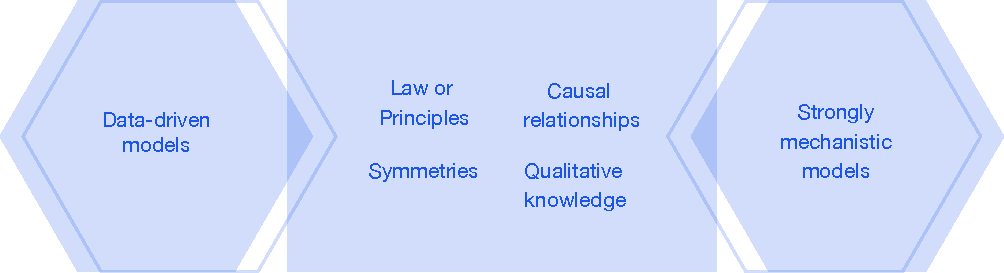
\includegraphics[width=0.8\textwidth]{media/figure-1.pdf}
\end{center}
\caption{Models along a spectrum from classical i.i.d models to strongly mechanistic differential equation models introduce aspects of causality and symmetries to create a continuum between mechanistic and data-driven worlds. Statistical or data-driven models are weakly mechanistic (i.e. they include smoothness assumptions or similar).}
\label{model-spectrum}
\end{figure}

At one end of that continuum, mechanistic models would obey known laws
or principles in a strongly deterministic way; at the other, statistical
models encode fewer assumptions and rely more on data. The addition of
invariances and symmetries, alongside other forms of domain knowledge,
allows bridging between these two model classes (Figure \ref{model-spectrum}). Models that
describe how much heat is absorbed by the oceans under conditions of
climate change, for example, should obey the laws of thermodynamics and
energy conservation. By encoding the domain knowledge that has yielded
these fundamental laws, such as the conservation of momentum or energy,
researchers can ensure the outputs of a machine learning model will have
a physically allowable expression. This encoding can come from
integrating equations, symmetries, or invariances into model design.
These encodings constrain the operation of a machine learning system to
align with the known dynamics of physical systems. The resulting models
might be expected to produce more accurate results, with smaller
generalisation errors, and with better out-of-distribution
generalisation.

\begin{figure}
\begin{center}
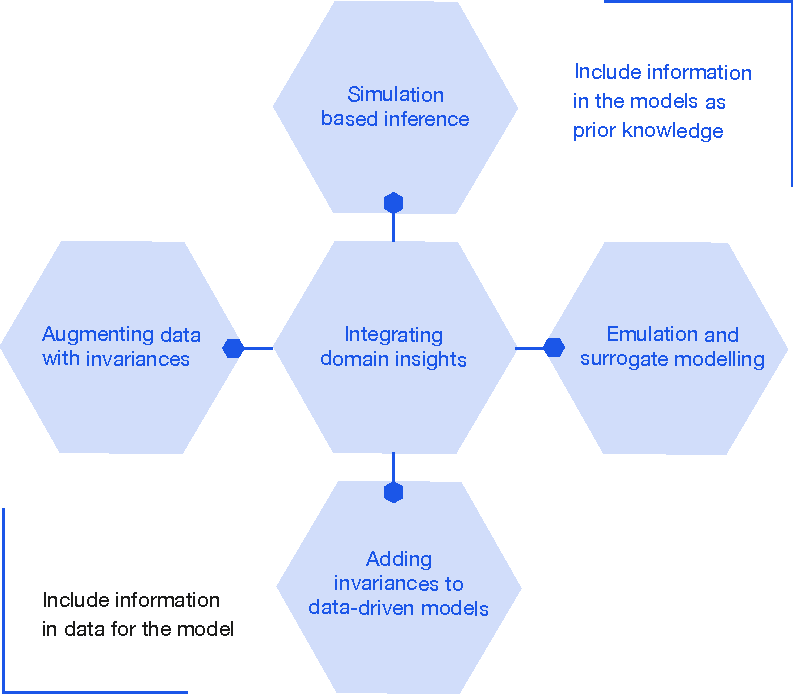
\includegraphics[width=0.8\textwidth]{media/figure-2.pdf}
\end{center}
\caption{Strategies for integrating domain insights: including information in data and including information as prior knowledge.}
\end{figure}

\subsection{Scientific centaurs}\label{scientific-centaurs}

Complementing modelling strategies to encode scientific knowledge are
deployment strategies to use AI in the lab. The lab has long provided a
physical hub for collaboration and knowledge-generation, its function
and form having remained broadly consistent across centuries of
scientific progress. Today, the digitisation of experimental equipment
and laboratory processes offers opportunities to integrate AI in
experimental design and create new virtual labs.

By combining data from measurement devices, simulations of laboratory
processes, and computational models of research or user objectives,
these virtual labs provide a digital sibling of in-person research
activities that can be used to optimise such activities. In drug
discovery, for example, virtual labs could accelerate the testing and
analysis processes that identify candidate drugs from potential drug
targets. Instead of relying on physical testing of such starting
molecules, multiple rounds of virtual testing can rapidly simulate the
processes of drug design, manufacture, testing, and analysis to assess
which starting molecules are more (or less) likely to be viable
candidate drugs \cite{Klami-virtual22}.
As a result, AI can help accelerate the research process.

Advances in machine learning methods to enable effective simulations,
causal modelling, and encoding pre-existing domain insights -- while
packaging such methods into usable toolkits -- are all necessary
foundations for such digital siblings. Moving from virtual laboratory to
`AI assistants' requires further advances in AI system design to create
AI agents that can elicit guidance or input from their domain experts.
Such agents would not only provide useful intuitions for scientific
modelling, but would serve as `scientific sidekicks', actively helping
researchers to drive their research.

This new type of AI assistant would combine the ability to model the
research problem of interest with the ability to model the goals and
preferences of their expert users, even when the user themselves might
not be able to clearly articulate those goals. As a starting point,
these systems would need to support forms of user interaction that can
extract user knowledge, leveraging this to identify appropriate courses
of action. To operate in contexts where user goals might be uncertain
and user behaviour might change in response to the outputs of the AI
system, these AI sidekicks will need insights from cognitive science,
studies of team decision-making, and new learning strategies based on
limited examples. The sophisticated user modelling so-created would
unlock new forms of human-AI collaboration; scientific centaurs that
combine both human and machine intelligence \cite{Celikok-best22}.

\subsection{Enabling communication across
domains}\label{enabling-communication-across-domains}

Underpinning these efforts to integrate pre-existing knowledge into the
design and deployment of AI systems is a feedback loop between domain
and machine learning research, in which each elicits from and feeds into
the other. This loop requires the ability to exchange knowledge and
insights across disciplines through interdisciplinary collaboration and
communication.

Matching model to user need requires shared understandings of the
research question at hand, the constraints -- whether from data,
compute, funding, or time and energy available -- that affect different
collaborators, and the user needs of the domain environment. While AI
researchers might be tempted to develop complex models, showcasing
assorted theoretical and methodological advances in the field, from a
domain perspective, a relatively `simple' model may seem preferable.
Collaborators need to be able to mutually explore what is possible,
while also considering what is useful.

To complete the loop, outputs from machine learning models need to feed
back into the application domain: insights from AI need to be accessible
in ways that allow the transfer of learning from model to user. This
implies some level of explainability. It is not sufficient for an AI
system to produce highly accurate results; those results must also be
interpretable by a domain researcher. As the complexity of AI systems
increases, however, understanding why these systems have produced a
particular result becomes increasingly challenging. While not an issue
for all machine learning methods, this complexity often results in
difficulties explaining the functioning of AI systems.

In response, AI researchers have developed a variety of different
methods to interrogate how AI systems work, or why a particular output
has been produced. Again, to understand which of these methods is
desirable in the context of a scientific application, researchers must
collaborate closely with domain experts. In the context of
pharmaceutical experiments where the aim is to measure how many target
cells are killed off at different dosages of a drug (or drug
combination), for example, researchers might be seeking to `sense-check'
how different drug dosages affect the model, before investigating
specific drugs more rigorously. In astronomical studies, researchers are
often working with high-dimensional datasets with many confounding
correlations. For example, gravitational waves are ripples in space-time
catalysed by the movement of massive bodies in space, such as planets or
stars \cite{NASA-gravitational}.
These invisible phenomena are studied at observatories across the
world,\footnote{See, for example, the LIGO project. Information
  available at:
  \url{https://www.ligo.caltech.edu}}
based on models to describe wave signals and the `noise' generated by
instruments that measure them \cite{Dax-gravitational21}.
Measurements of gravitational waves can be used to infer the properties
of black holes that create them, such as their location, mass, and spin,
using simulation-based inference to characterise the source of a wave,
given the data that detects it. To make such methods more efficient than
existing analytical tools, researchers need to take into account the
structure that sits underneath it: for example, gravitational wave
detectors are located across the globe, and their location affects the
angle at which they detect waves hitting the Earth. This structure can
be exploited through data sampling strategies to help make machine
learning more efficient \cite{Dax-gravitational21}. An alternative, however, is to
use deterministic models that already reflect relevant physical
laws \cite{Bodin-black21}. Across these approaches,
software packages play an important role in enabling communication and
dissemination of methods for wider use.\footnote{See, for example:
  \url{https://lscsoft.docs.ligo.org/bilby/}}

\subsection{Directions}\label{directions-2}

New modelling approaches and mathematical innovations offer exciting
opportunities to integrate domain knowledge, symmetries and invariances
into AI systems \cite{Villar-dimensionless22}.
Integration can be achieved in different ways:

\begin{itemize}
\item
  Data augmentation can help exploit invariances and symmetries,
  resulting in improved model performance, by including in the data
  domain knowledge for a model to ingest.
\item
  Symmetries can be embedded in the design of deep learning systems, for
  example by using the same convolutional filters in different locations
  of an image, CNNs can leverage translation and rotation symmetries.
\item
  Latent force models allow representations of known symmetries
  alongside probabilistic factors, enabling integration of mechanistic
  models with unknown forces \cite{Ward-blackbox20}.
\item
  Architectural features can restrict model focus to outputs that
  satisfy symmetries, for example using weight sharing, irreducible
  representations, or invoking symmetries as constraints.\footnote{See,
    for example: \cite{Kondor-generalization18,Maron-invariant18,Dym-universality20}}
\item
  Loss functions can be deployed to penalise predictions that fail to
  satisfy physical constraints or symmetries.
\end{itemize}

In the process, emerging mathematical questions include: how can AI
learn invariances from data? And is it possible to quantify the
performance gain achieved through this?

Research to develop AI assistants in the lab raises interesting
questions about learning strategies and human-machine collaboration.
These AI agents would need to be able to learn how to assist another
agent, in a multi-agent decision-making scenario, where goals might be
unclear, uncertain, or changeable. To tackle this challenge:

\begin{itemize}
\item
  Decision-making with delayed reward or zero-shot learning can help
  agents solve tasks when there is little or nothing known about the
  reward function, and no previous behaviour to learn from.
\item
  Interactive knowledge elicitation \cite{Sundin-improving18},
  combining prior knowledge from cognitive science with learning from
  data \cite{Kangasraasio-parameter19},
  and generative user models \cite{DePeuter-toward21}
  can support more effective interactions between user and machine.
\end{itemize}

Across these areas, care is needed in the design of the points of
interaction between human and AI system. A core question here is: how
can AI researchers extract domain knowledge from relevant experts and
integrate it into a machine learning model? Insights from human-machine
interaction studies and collaborative decision-making systems are
necessary to create effective interfaces between human and machine,
based on factors such as:

\begin{itemize}
\item
  What forms of visualisation are helpful for human users?
\item
  What types of interpretability or explainability are needed for a user
  to achieve their desired interactions?
\item
  What might be the unintended consequences of human-machine
  interaction, such as over-confidence in results or over-reliance on
  the AI system?
\item
  What `theory of mind' is needed to anticipate how human users might be
  likely to respond to an AI system?
\end{itemize}

A challenge in these interactions is that much of the relevant knowledge
held by the domain expert might be qualitative: an intuition of how a
system works, developed over a long period of study, rather than
quantifiable insights.

\subsection{Talks given during this workshop session}

\abstracttitle{Virtual laboratories for science, assisted by collaborative AI}
\abstractauthor[Samuel Kaski]{Samuel Kaski (Aalto University, FI)}
\license

I introduced two ideas: virtual laboratories for science, aiming to introduce an interface between algorithms and domain science that enables AI-driven scale advantages, and AI-based ‘sidekick’ assistants, able to help other agents research their goals, even when they are not able to yet specify the goal explicitly, or it is evolving. Such assistants would ultimately be able to help human domain experts run experiments in the virtual laboratories. I invited researchers to join the virtual laboratory movement, both domain scientists in hosting a virtual laboratory in their field and methods researchers in contributing new methods to virtual laboratories, simply by providing compatible interfaces in their code. For developing the assistants, I introduced the basic problem of agents that are able to help other agents reach their goals, also in zero-short settings, formulated the problem, and introduced solutions in the simplified setting of prior knowledge elicitation, and in AI-assistted decision and design tasks.

\abstracttitle{Making data analysis more like classical physics}
\abstractauthor[David W. Hogg]{David W. Hogg (New York University, US)}
\license

The laws of physics are very structured: They involve coordinate-free forms, they are equivariant to a panoply of group actions, and they can be written entirely in terms of dimensionless, invariant quantities. We find that many existing machine-learning methods can be very straightforwardly modified to obey the rules that physical law must obey; physics structure can be implemented without big engineering efforts. We also find that these modifications often lead to improvements in generalization, including out-of-sample generalization, in natural-science contexts. We have some intuitions about why.

The second example is work by Dan Sheldon on analysis of doppler radar
to extract bird biomass and motion. The radar measures the radial
velocity modulo a constant (i.e., the velocity wraps around to zero).
Previous work had attempted to "unwrap" the data using heuristics. Dan
instead incorporated the modulus operation into the likelihood function
and then developing an algorithm for maximizing this somewhat nasty
likelihood. The result has revolutionized radar analysis and has been
deployed in the BirdCast product from the Cornell Lab of Ornithology.

The third example is the species occupancy model introduced by MacKenzie
et al (2002). When human observers conduct wildlife surveys, they may
fail to detect a species even though the species is present. The
occupancy model combines this detection probability with a habitat
model. However, the expressiveness of the two models (detection and
habitat) must be carefully controlled. Rebecca Hutchinson and I learned
this when we tried to replace the linear logistic regression models with
boosted trees.

In all cases, downstream use of the estimates that come from such data
collection models must be aware of the measurement uncertainties. How
can we correctly quantify those uncertainties and incorporate them in
the downstream analysis? Maybe there are lessons ecologists can learn
from physicists?

\abstracttitle{Latent force models}
\abstractauthor[Mauricio A. \'Alvarez]{Mauricio A. \'Alvarez (University of Manchester, GB)}
\license

A latent force model is a Gaussian process with a covariance function inspired by a differential operator. Such a covariance function is obtained by performing convolution integrals between Green's functions associated with the differential operators, and covariance functions associated with latent functions. Latent force models have been used in several different fields for grey box modelling and Bayesian inversion. In this talk, I will introduce latent force models and several recent works in my group where we have extended this framework to non-linear problems.

\abstracttitle{Translating mechanistic understandings to stochastic models}
\abstractauthor[Carl Henrik Ek]{Carl Henrik Ek (University of Cambridge, GB)}
\license

Statistical learning holds the promise of being the glue that allows us to improve knowledge parametrised explicitly by a mechanistic model with implicit knowledge through empirical evidence. Statistical inference provides a narrative of how to integrate these two sources of information leading to an explanation of the empirical evidence in "light" of the explicit knowledge. While the two sources of knowledge are exchangeable in terms of predictive performance they are not if our focus is that of statistical learning as a tool for science where we want to derive new knowledge.

In this talk we will focus on challenges associated with translating our mechanistic understanding into stochastic models such that they can be integrated with data. In particular, we will focus on the challenges of translating composite knowledge. We will show how these structures and the computational intractabilities they lead to make knowledge discovery challenging. 

The perceived `success' of machine learning comes from application where we have large volumes of data such that only simple and generic models are needed in order to regularise the problem. This means that much of the progress that have been made with predictive models are challenging to translate into useful mechanisms for scientific applications. In this talk we will focus on challenges associated with translating our mechanistic understanding into stochastic models such that they can be integrated with data. In specific we will focus on the challenges of translating composite knowledge. We will show how these structures and the computational intractabilities they lead to makes knowledge discovery challenging. We will discuss properties that we desire from such structures and highlight the large gap that exists with current inference mechanism.
